% !TEX root = algo-quicksheet.tex
\chapter{Tree}

\section{Binary Tree}
\subsection{Recursion}
The basic opeartion with tree is recursion. 

\runinhead{Information Propagation.} To propagate information:
\begin{itemize}
\item To propagate children's information to current node $\Ra$ use return values of recursion calls.
\item To propagate current node's information to children $\Ra$ use parameters for recursion calls
\item To propagate current node's or children's information to global memory $\Ra$ use \pyinline{self} or \pyinline{global} vars. 
\end{itemize}

\runinhead{Condition checking.} To check the predicate, we normally check the predicate upon entering the recursion calls for trees as terminal condition. For graphs, we normally check the predicate before entering the recursion calls. 

\subsection{Basic Operations}
\runinhead{Get parent ref.} To get a parent reference (implicitly), \textit{return the Node} of the current recursion function to its parent to maintain the path. Sample code:
\begin{python}
# delete minimum node in the BST
def delete_min(x: Node) -> Node:
    if not x.left:
        return x.right
    x.left = delete_min(x.left)
    return x
\end{python}

\runinhead{Max depth.} Propagate depth information to children. 
\begin{python}
def get_depth(self, cur, depth):
    if not cur:
        return depth

    return max(
        self.get_depth(cur.left, depth+1), 
        self.get_depth(cur.right, depth+1),
    )
\end{python}

\runinhead{Max depth.} Propagate depth information back to current node / parent. 

\begin{python}
def dfs(self, cur):
    if not cur:
        return -1  # leaves index start from 0

    depth = 1 + max(
        self.dfs(cur.left), 
        self.dfs(cur.right),
    )
    
    # do something
     
    return depth
\end{python}

Application: leaf by leaf traversal by height. 
\begin{python}
def dfs(self, cur, leaves):
    if not cur:
        return -1  # leaves index start from 0

    height = 1 + max(
        self.dfs(cur.left, leaves), 
        self.dfs(cur.right, leaves),
    )
    if height >= len(leaves):
        leaves.append([])  # grow

    leaves[height].append(cur.val)
    return height
\end{python}

\runinhead{Min depth.} Definition of min depth, lowest depth of leaf node. 

Notice, that the additional checks are necessary of missing either right or left child.
\begin{python}
def probe(self, cur, depth):
    if not cur: 
        return depth
    elif cur.right and not cur.left: 
        return self.probe(cur.right, depth+1)
    elif cur.left and not cur.right: 
        return self.probe(cur.left, depth+1)
    else: 
        return min(
            self.probe(root.left, depth+1), 
            self.probe(root.right, depth+1),
        )
\end{python}
Alternatively,
\begin{python}
def minDepth(cur) -> int:
  if not cur:
    return 0  
  if not cur.left and not cur.right:
    return 1

  left = minDepth(cur.left) if cur.left else sys.maxsize
  right = minDepth(cur.right) if cur.right else sys.maxsize
  return 1 + min(left, right)
\end{python}
\runinhead{Construct path from root to a target.} To search a node in binary tree (not necessarily BST), use dfs:
\begin{python}
def dfs(self, cur, target, path):
    # post function call check
    if not cur:
      return        
    if self.found:
      return 

    path.append(cur)
    if cur == target:
        self.found = True

    self.dfs(cur.left, target, path)
    self.dfs(cur.right, target, path)
    if not self.found:
        path.pop()  # 1 pop() corresponds to 1 append()
\end{python}
The \pyinline{found} is an obj's field of boolean to keep it referenced by all calling stack. 

\runinhead{Lowest common ancestor.} In BST, the searching is straightforward. 
\begin{python}
def find_lca(self, cur, p, q):
    if p.val > cur.val and q.val > cur.val:
        return self.find_lca(cur.right, p, q)
    if p.val < cur.val and q.val < cur.val:
        return self.find_lca(cur.left, p, q)
    return cur
\end{python}

Method 1: In general binary tree, construct the path from root to $node_1$ and $node_2$ respectively, and \textbf{diff} the two paths. Time complexity: $O(\lg n)$, space complexity: $O(\lg n)$. 

Method 2: If the parent pointer is provided, it is possible to reduce the space complexity to $O(1)$, by using two pointers: 
\begin{python}
def find_lca(n1, n2):
    if not n1 or not n2:
        return None 
        
    d1, d2 = depth(n1), depth(n2)
    if d2 < d1:
        return find_lca(n2, n1)  # swap
        
    # move to the same depth 
    for _ in range(d2-d1):
        n2 = n2.parent  

    while n1 and not n1 == n2:  
        n1 = n1.parent
        n2 = n2.parent
        
    return n1
\end{python}

Method 3: In general bindary tree and to achieve \hl{$O(1)$ space}, bottom up to find the first node that has $p, q$ in its left and right substrees simultaneously.

A node is lca of itself.

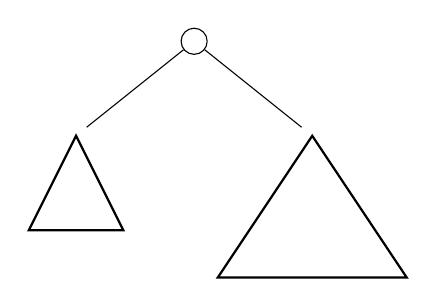
\begin{tikzpicture}[level distance=1.2cm, % reduced from 2.5cm
  every node/.style={draw, circle},
  level 1/.style={sibling distance=3cm}]

% Root node
\node (root) {}

% Left and right subtree placeholders
child {node[draw=none] (left) {}}
child {node[draw=none] (right) {}};

% Draw left triangle (subtree)
\draw[thick] (left) ++(-0.6,-1.2) -- ++(0.6,1.2) -- ++(0.6,-1.2) -- cycle;

% Draw right triangle (subtree)
\draw[thick] (right) ++(-1.2,-1.8) -- ++(1.2,1.8) -- ++(1.2,-1.8) -- cycle;

\end{tikzpicture}
\begin{python}
def find_either(self, node, p, q):
    if node is None:
        return None
    
    # a node is lca of itself
    if node == p or node == q:
        return node
    
    left = self.find_either(node.left, p, q)
    right = self.find_either(node.right, p, q)
    
    # lca
    if left and right:
    	self.ans = node
        return node
    
    return left if left else right
\end{python}

Method 4: \pyinline{count} can be extended to find the LCA of a set of nodes
\begin{python}
def count(self, node, p, q):
    if not node:
        return 0

    l = self.count(node.left, p, q)
    r = self.count(node.right, p, q)
    m = 1 if node in (p, q) else 0
    ret = l + m + r
    if ret == 2 and not self.ans:
        # only keep the lowest
        self.ans = node
    return ret
\end{python}

\runinhead{Find all paths.} Find all paths from root to leafs. 

For every currently visiting node, add itself to path; search left, search right and pop itself. Record current result when reaching the leaf.
\begin{python}
def dfs(self, cur, path, ret):
    if not cur:
        return

    path.append(cur)
    if not cur.left and not cur.right:
        ret.append("->".join(map(repr, path)))

    self.dfs(cur.left, path, ret)
    self.dfs(cur.right, path, ret)
    path.pop()  # 1 append 1 pop
\end{python}

\runinhead{Leftmost node.} Find the leftmost node. 
\rih{Core Clues:}
\begin{enumerate}
\item Greedy go left? $\Ra$ a counter case $\Ra$ need to check both sides.
\end{enumerate}
\begin{python}
def leftmost(self, cur, offset):
    # offset from center 0, negative means left side. 
    if not cur:
        return offset
    return min(
        self.leftmost(cur.left, offset-1), 
        self.leftmost(cur.right, offset+1),
    )
\end{python}

Rightmost node can be similarly found.

\runinhead{Diameter of a tree (graph).} The diameter of a tree $\equiv$ longest path in the tree.  

Core clues:
\begin{enumerate}
\item Longest path $\Ra$ Intuitily, we need to find one end of the edge, and then find the other end.
\item \rih{Edge} $\Ra$ Edge to edge, furtherest to frutherest.
\item \rih{Find one end of the edge} $\Ra$ start from any vertex, bfs to reach the farthest leaf.
\item \rih{Find the other end} $\Ra$ start from this leaf node, bfs to reach the other farthest leaf. 
\end{enumerate}
\begin{python}
_, _, last = self.bfs(0, G)
level, pis, last = self.bfs(last, G)

def bfs(self, s, G) -> Tuple[int, List[Vertex], Vertex]:
    # bfs
    visited = defaultdict(bool)
    # predecessor 
    pis = defaultdict(lambda: -1)
    last = s  # last visited
    level = 0
    q = [s]
    while q:
        new_q = []
        for e in q:
            last = e
            visited[e] = True
            for nbr in G[e]:
                if not visited[nbr]:
                    pis[nbr] = e
                    new_q.append(nbr)

        q = new_q
        level += 1

    return level, pis, last
\end{python}

Alternatively, use tree:
\begin{python}
def diameterOfBinaryTree(self, root):
    self.ret = -1
    self.dfs(root)
    return self.ret        

def diam(self, subroot):
    # get the longest path to any leaf node
    if not subroot:
        return 0
    
    left = self.diam(subroot.left)
    right = self.diam(subroot.right)
    self.ret = max(self.ret, left + right)
    return max(left, right) + 1  # +1 to make progress
\end{python}


\runinhead{Distance to its leaves.} Counstruct a map of distance $\ra$ count. The distance is from current node to leaves, and the count is number of leaves. 

\rih{Core Clues:}
\begin{enumerate}
\item Objective: maintain a map from distance $\ra$ to count.
\item Each: each node has a map of distance $\Ra$ we need return value on the recursion stacks rather than a value passed in the recursion. 
\item Leaf: the leaf node has a base case - distance to itself is 0
\end{enumerate}

\begin{python}
def distances(self, node) -> dict:
    counts = defaultdict(int)  # distance -> count
    if not node:
        return counts
    
    if not node.left and not node.right:
        counts[0] = 1
        return counts

    left = self.distances(node.left)
    right = self.distances(node.right) 
    for k, v in left.items():
        for K, V in right.items():
            self.consume(k, K, v, V)
    
    # merge
    for k, v in left.items():
        counts[k+1] += v
    for k, v in right.items():
        counts[k+1] += v

    return counts
\end{python}

\runinhead{Max Distance to a target node.} Node to node distance within a tree. Find the maximum distane from a node to a target node. The start node and cabe any node, $\exists node$. Not necessarily from the root.

\begin{center}
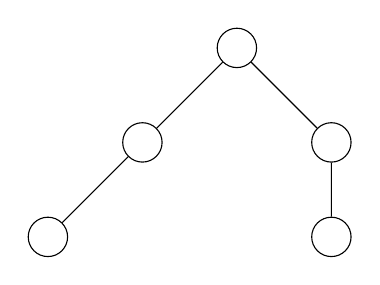
\begin{tikzpicture}[
scale=0.6,
% transform shape,
every node/.style={circle,draw,minimum size=5mm,inner sep=0pt},
level distance=1.2cm
]
  % nodes
  \node (root) at (0,0) {};
  \node (L1)   at (-2,-2) {};
  \node (L2)   at (-4,-4) {};
  \node (R1)   at ( 2,-2) {};
  \node (R2)   at ( 2,-4) {};
  % edges
  \draw (root)--(L1)--(L2);
  \draw (root)--(R1)--(R2);
\end{tikzpicture}
\end{center}

\rih{Core Clues:}
\begin{itemize}
\item Convert the tree to graph, and BFS from the target node is trivial, but it requires 2 passes
\item To solve it in 1 pass, we need to dfs:
\begin{enumerate}
\item Maintain a depth from current node to the target node \textbf{or} leaf.
\item If root is the target $\Ra$ get max depth from left and right subtrees 
\item If target is on one (e.g. left) side of the root $\Ra$ depth to the target + right depth to leaf
\end{enumerate}
\end{itemize}

\begin{python}
self.maxa 

# depth from a node to target or leaf
def dfs(self, cur, target) -> bool, int:
    if not cur:
        return False, -1
    
    l_found, l_depth = self.dfs(cur.left, target)
    r_found, r_depth = self.dfs(cur.right, target)
    
    if cur.val == target:
        depth = max(l_depth, r_depth) + 1
        self.maxa = max(self.maxa, depth)
        return True, 0

    if l_found:
        dist = (l_depth + 1) + (r_depth + 1)   # from child to cur
        self.maxa = max(self.maxa, dist)
        return l_found, l_depth + 1
        
    if r_found:
        dist = l_depth + r_depth + 2  # from child to cur
        self.maxa = max(self.maxa, dist)
        return r_found, r_depth + 1
    
    return False, depth
\end{python}

\runinhead{Longest Consecutive Sequence.} A consecutive path is a path where the values of the consecutive nodes in the path differ by one. This path can be either increasing or decreasing.

\rih{Core Clues}:
\begin{enumerate}
\item Break down the problem: treat asc and dec separately
\item Let $inc$ with the length of increasing subarray ending at $node$
\end{enumerate}

\begin{python}
class Solution:
  def longestConsecutive(self, root) -> int:
    self.ret = 0
    self.dfs(root)
    return self.ret
  
  def dfs(node) -> Tuple[int, int]:
    if not node:
      return 0, 0  # inc, dec

    ginc = gdec = 1

    linc, ldec = dfs(node.left)
    rinc, rdec = dfs(node.right)

    inc = dec = 1
    if node.left and node.left.val == node.val + 1:
        inc = max(inc, linc + 1)
    if node.right and node.right.val == node.val - 1:
        dec = max(dec, rdec + 1)
    self.ret = max(self.ret, inc + dec - 1)
    ginc = max(ginc, inc)
    gdec = max(gdec, dec)
    
    # mirrored    
    inc = dec = 1
    if node.left and node.left.val == node.val - 1:
        dec = max(dec, ldec + 1)
    if node.right and node.right.val == node.val + 1:
        inc = max(inc, rinc + 1)     
    self.ret = max(self.ret, inc + dec - 1)
    ginc = max(ginc, inc)
    gdec = max(gdec, dec)
    
    return ginc, gdec
\end{python}

\subsection{Vertical Traversal}
\begin{figure}[hbtp]
\centering
\subfloat{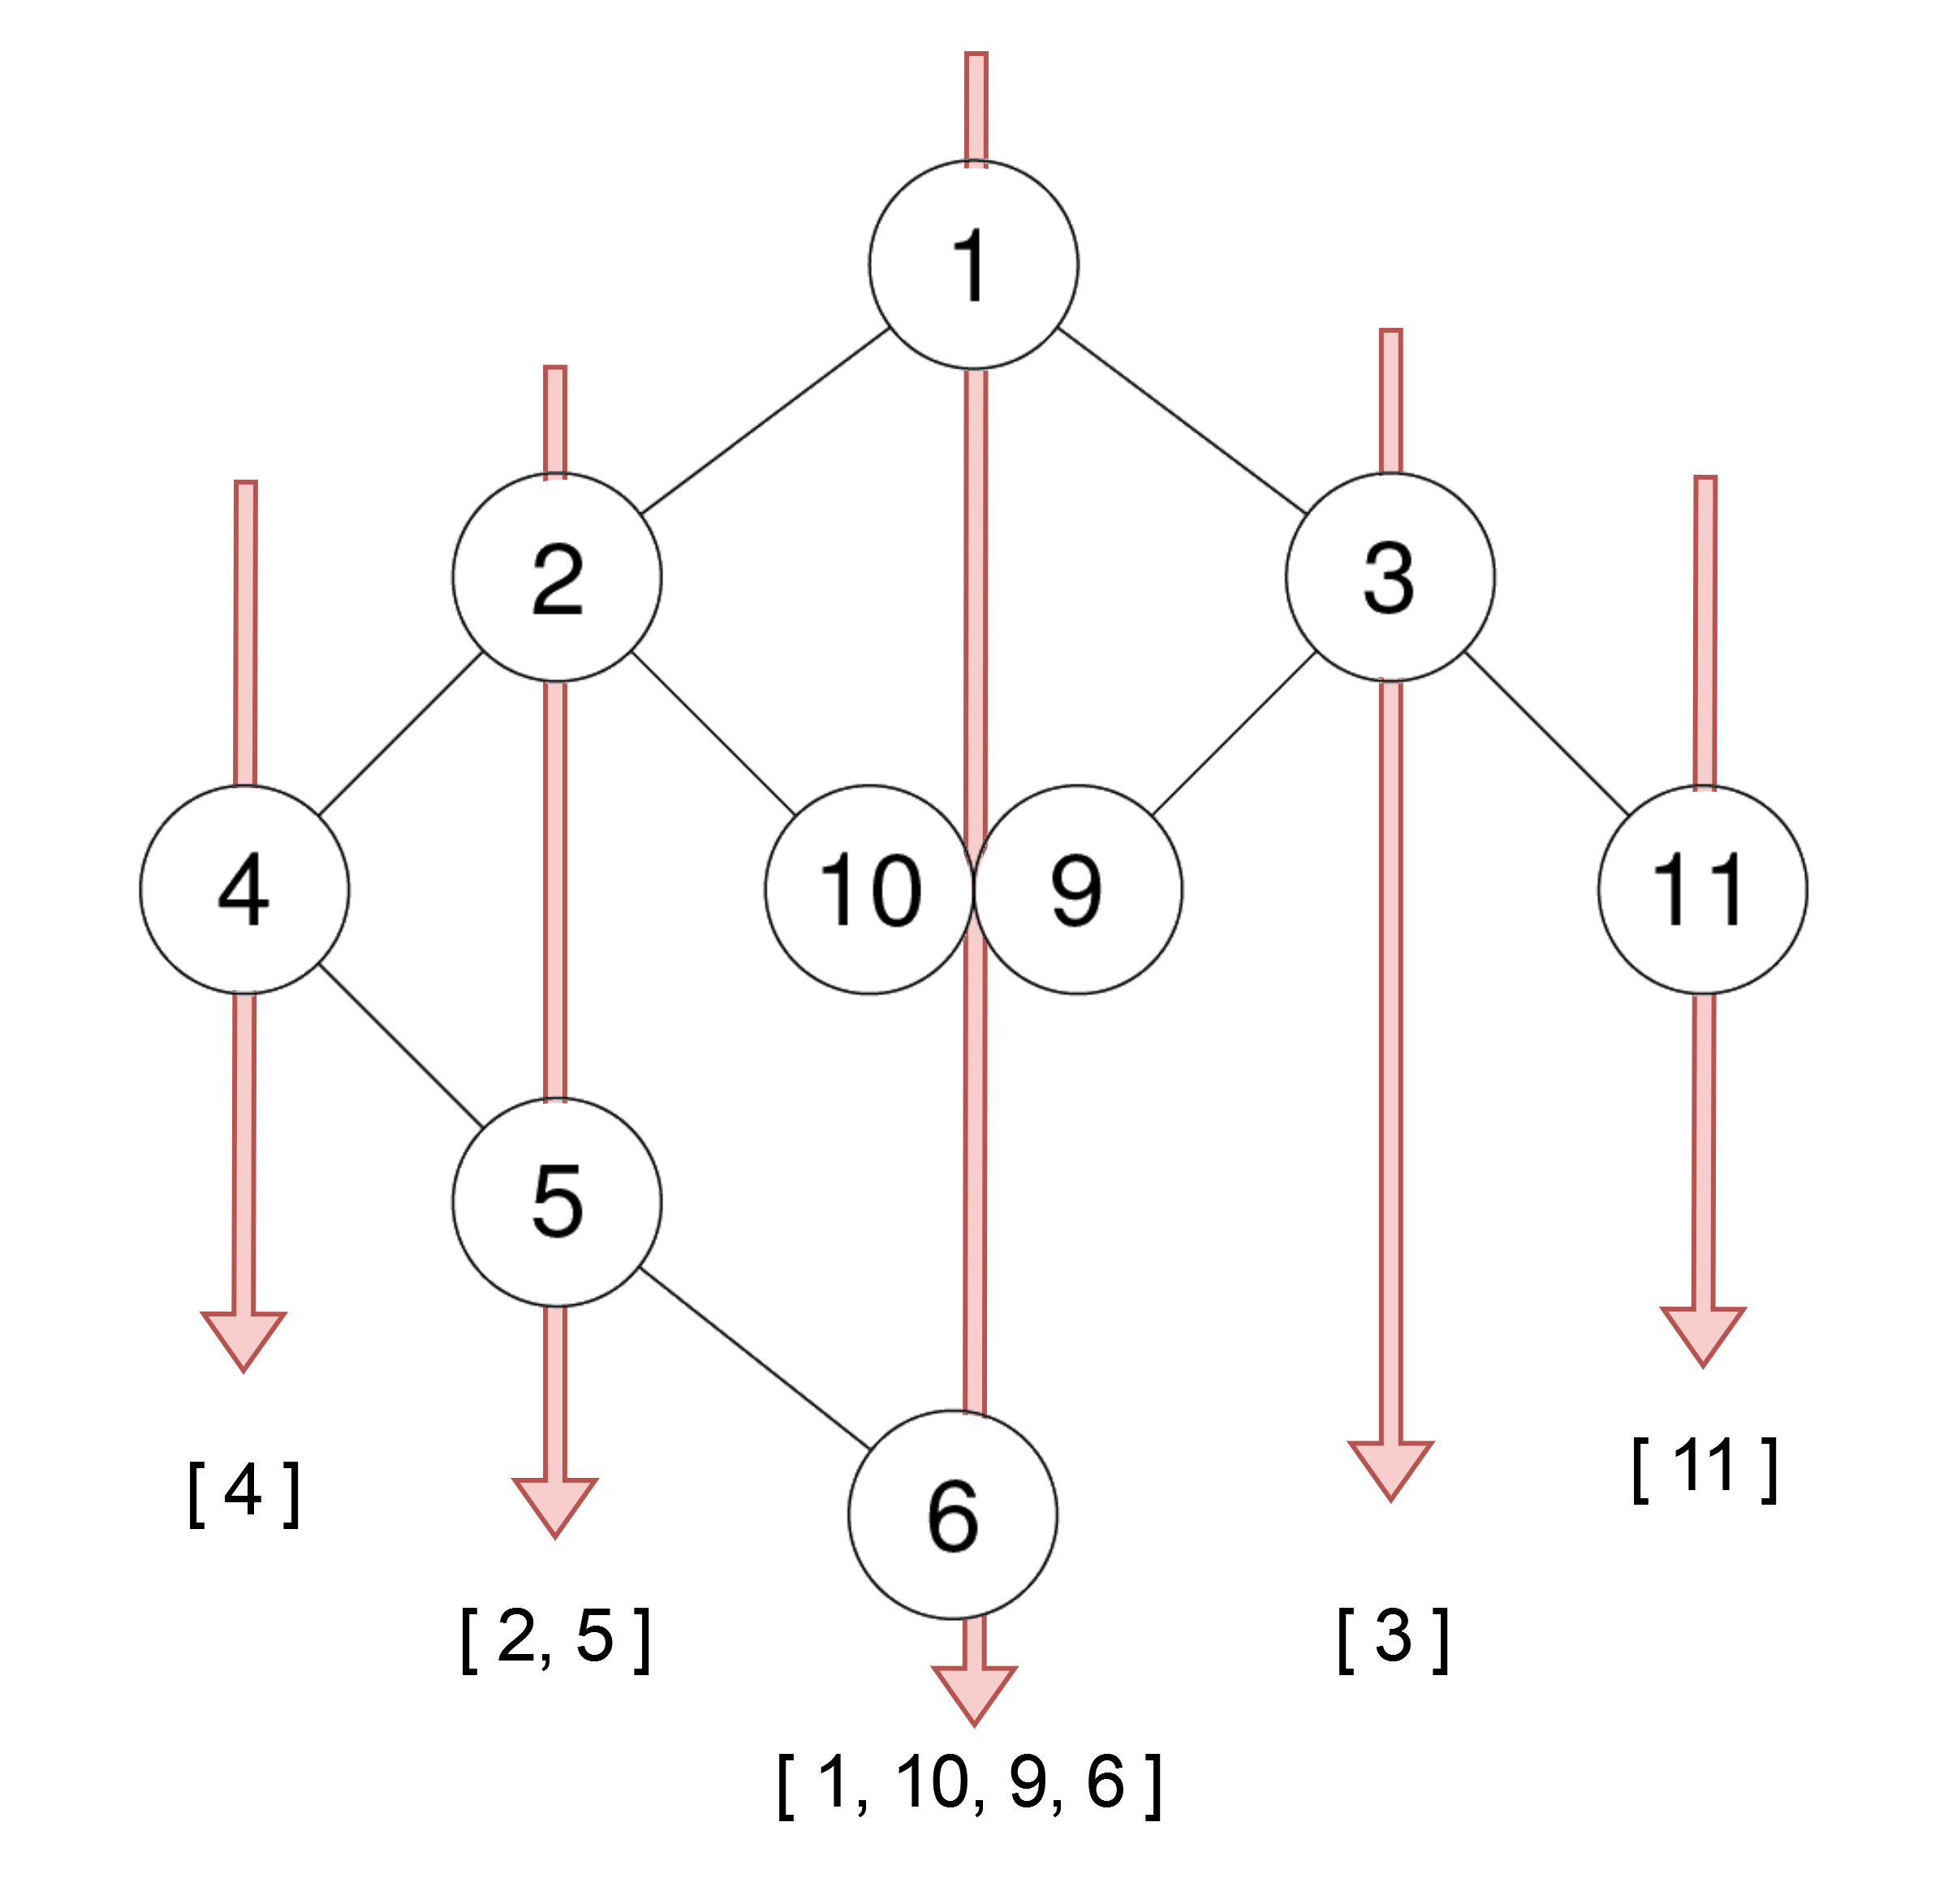
\includegraphics[height=2.2in]{vertical_traversal}}
\caption{Vertical Traversal}
\label{fig:vertical_traversal}
\end{figure}
\runinhead{Core Clues}:
\begin{enumerate}
\item Vertical traversal $\Ra$ columns, starting from root as 0, there can be negative and positive offset
\item Order within each column $\Ra$ level by level, thus BFS required
\end{enumerate}
\begin{python}
def verticalOrder(self, root):
    l = self.leftmost(root, 0)
    r = self.rightmost(root, 0)

    ret = [[] for _ in range(r-l-1)]
    self.bfs(root, -l-1, ret)
    return ret

def bfs(self, cur, col, ret):
    q = []
    if cur:
        q.append((cur, col))

    while q:
        new_q = []
        for e in q:
            v, c = e
            ret[c].append(v.val)
            if v.left:
                new_q.append((v.left, c-1))
            if v.right:
                new_q.append((v.right, c+1))

        q = new_q

def leftmost(self, cur, col):
    if not cur: 
        return col
    return min(
        self.leftmost(cur.left, col-1), 
        self.leftmost(cur.right, col+1)
    )

def rightmost(self, cur, col):
    if not cur: 
        return col
    return max(
        self.rightmost(cur.left, col-1), 	
        self.rightmost(cur.right, col+1),
    )
\end{python}

If using \pyinline{defaultdict(list)} with negative/positive offset, the order prefers left.
\begin{python}
def verticalOrder(self, root) -> List[List[int]]:
    self.lists = defaultdict(list)
    self.dfs(root, 0)
    # re-adjust
    floor = min(self.lists.keys())
    ret = [[] for _ in range(len(self.lists))]
    for k, v in self.lists.items():
        ret[k - floor] = v
    return ret

def dfs(self, cur, offset):
    if not cur:
        return 

    self.lists[offset].append(cur.val)
    self.dfs(cur.left, offset-1)
    self.dfs(cur.right, offset+1)
\end{python}
\subsection{Morris Traversal} 
Traversal with O(1) space. \footnote{\href{http://www.cnblogs.com/AnnieKim/archive/2013/06/15/MorrisTraversal.html}{ref}}
Three ways of traversal: in-order, pre-order, post-order.
Time complexity $O(3n).$ Find \pyinline{pre} twice, traverse \pyinline{cur} once.
\begin{figure}[hbtp]
\centering
\subfloat{\includegraphics[height=1.2in]{morris_time}}
\caption{Morris traversal time complexity}
\label{fig:morrisTime}
\end{figure}

Core:
\begin{enumerate}
\item Threading from \textbf{in-order} predecessor to \pyinline{cur}.
\item In-order consumes the \pyinline{cur} when going right, pre-order when going left, post-order consumes the left subtree path when going right. 
\end{enumerate}
\subsubsection{In-order}
Given the current node \pyinline{cur}, we know the next child node. But how does its predecessor knows \pyinline{cur}? Assign the current node's in-order predecessor's right child to itself (threading). Two ptr \pyinline{cur}, \pyinline{pre}. 

Process:
\begin{enumerate}
\item If no left, \textit{consume} \pyinline{cur}, go right 
\item If left, find in-order predecessor \pyinline{pre}
\begin{enumerate}
\item If not threaded (i.e. no \pyinline{pre} right child), assign it to \pyinline{cur}; go left
\item If threaded, \textit{consume} \pyinline{cur}, go right. ($\equiv$ no left). 
\end{enumerate}
\end{enumerate}

\begin{figure*}[!htb]
\centering
\subfloat{\includegraphics[height=2.45in]{morris_inorder}}
\caption{Morris in-order traversal}
\label{fig:morrisInorder}
\end{figure*}

Code:
\begin{python}
def morris_inorder(self, root):
    cur = root
    while cur:
        if not cur.left:
            self.consume(cur)
            cur = cur.right
        else:  
            pre = cur.left
            while pre.right and pre.right != cur:
                pre = pre.right

            if not pre.right:
                pre.right = cur
                cur = cur.left
            else:
                pre.right = None
                self.consume(cur)  # when pop the thread
                cur = cur.right
\end{python}
\subsubsection{Pre-order}
Similar to in-order. Pre-order consume the current node when setting the thread rather than removing the thread as in in-order.

Process:
\begin{enumerate}
\item If no left, \textit{consume} \pyinline{cur}, go right 
\item If left, find in-order predecessor \pyinline{pre}
\begin{enumerate}
\item If no thread (i.e. no \pyinline{pre} right child), assign it to \pyinline{cur}; \textit{consume} \pyinline{cur}, go left
\item If thread, go right. ($\equiv$ no left, but no \textit{consume}, since consume before). 
\end{enumerate}
\end{enumerate}
Code:
\begin{python}
def morris_preorder(self, root):
    cur = root
    while cur:
        if not cur.left:
            self.consume(cur)
            cur = cur.right
        else:
            pre = cur.left
            while pre.right and pre.right != cur:
                pre = pre.right

            if not pre.right:
                pre.right = cur
                self.consume(cur)  # when set the thread
                cur = cur.left
            else:
                pre.right = None
                cur = cur.right
\end{python}
\subsubsection{Post-order}
More tedious but solvable. The process is also similar to in-order.

Process:
\begin{enumerate}
\item Set a temporary var \pyinline{dummy.left = root}
\item If no left, go right
\item If left, find the in-order predecessor \pyinline{pre} in left tree
\begin{enumerate}
\item If no thread, set \pyinline{right = cur} thread; go left.
\item If thread,  set \pyinline{right = None}, reversely \textit{consume} the path from \pyinline{cur.left} to \pyinline{pre}; go right.
\end{enumerate}
\end{enumerate}
\begin{figure*}[!htb]
\centering
\subfloat{\includegraphics[height=2.8in]{morris_postorder}}
\caption{Morris post-order traversal}
\label{fig:morrisInorder}
\end{figure*}
Code:
\begin{python}
def morris_postorder(self, root):
    dummy = TreeNode(0)
    dummy.left = root
    cur = dummy
    while cur:
        if not cur.left:
            cur = cur.right
        else:
            pre = cur.left
            while pre.right and pre.right != cur:
                pre = pre.right

            if not pre.right:
                pre.right = cur
                cur = cur.left
            else:
                pre.right = None
                self.consume_path(cur.left, pre)
                cur = cur.right

def _reverse(self, fr, to):
    """Like reversing linked list"""
    if fr == to: return
    cur = fr
    nxt = cur.right
    while cur and nxt and cur != to:
        nxt.right, cur, nxt = cur, nxt, nxt.right

def consume_path(self, fr, to):
    self._reverse(fr, to)

    cur = to
    self.consume(cur)
    while cur != fr:
        cur = cur.right
        self.consume(cur)

    self._reverse(to, fr)
\end{python}

\subsection{Zig Zag Traversal}
To zig zag traverse a tree, maintain a \pyinline{is_left} to determine direction. 

\runinhead{Find the longest zig zag path.} starting from any node in the tree. 

\rih{Core Clues:}
\begin{enumerate}
\item To determine direction $\Ra$ use \pyinline{is_left}
\item To check every node $\Ra$ restart the path with the current node. 
\end{enumerate}
\begin{python}
def longestZigZag(self, root):
    self.maxa = 0
    self.dfs(root, True, 0)
    self.dfs(root, False, 0)  # redundant
    return self.maxa - 1

def dfs(self, node, is_left, l):
    if not node:
        return

    l += 1
    self.maxa = max(self.maxa, l)
    
    if is_left:
        self.dfs(node.right, False, l)
        # restart with the current node
        self.dfs(node.left, True, 1)
    else:
        self.dfs(node.left, True, l)
        # restart with the current node
        self.dfs(node.right, False, 1)
\end{python}

Although in if-else statement, the code is the same, but the structure shows the logic.

\runinhead{Binary Tree Serialization and Deser.} 
\begin{center}
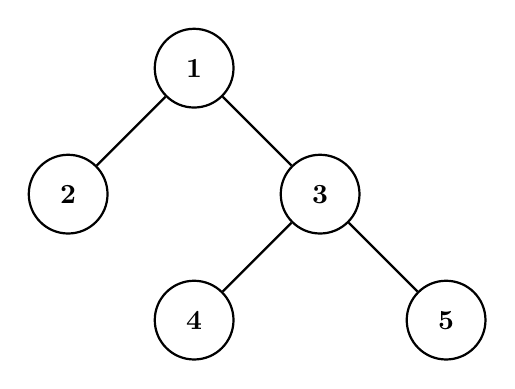
\begin{tikzpicture}[
	scale=0.8,
    every node/.style={draw,circle,minimum size=10mm,thick},
    node font=\bfseries,
    level/.style={sibling distance=32mm, level distance=18mm}
]
% coordinates for a simple diagonal layout
\node (n1) at (0,0) {1};
\node (n2) at (-2,-2) {2};
\node (n3) at ( 2,-2) {3};
\node (n4) at ( 0,-4) {4};
\node (n5) at ( 4,-4) {5};

\draw[thick] (n1) -- (n2);
\draw[thick] (n1) -- (n3);
\draw[thick] (n3) -- (n4);
\draw[thick] (n3) -- (n5);
\end{tikzpicture}
\end{center}
Serialized:
\begin{python}
[1,2,3,null,null,4,5,null,null,null,null]
\end{python}
\begin{enumerate}
\item Go through serialization by BFS. 
\item Ser by BFS can be either post-order or pre-order. It is straightforward.
\item Deser by BFS, to know the parent $\Ra$ it has to be pre-order BFS (encode before enqueue the $q$).
\end{enumerate}
\begin{python}
class Codec:
  def serialize(self, root):
    if not root:
      return "null"

    ret = [str(root.val)] # add result when enqueue
    q = [root]
    while q:
      new_q = []
      for cur in q:
        if cur.left:
          new_q.append(cur.left)
        ret.append(self.encode(cur.left))
        
        if cur.right:
          new_q.append(cur.right)
        ret.append(self.encode(cur.right))

      q = new_q

    return ",".join(ret)

  def deserialize(self, data):
    lst = data.split(",")
    root = self.decode(lst[0])  # decode when push in queue

    q = [root]
    i = 1  # simple BFS from q won't work
    while q:
      new_q = []
      for cur in q:
        if i < len(lst):
          cur.left = self.decode(lst[i])
          i += 1
          if cur.left:
            new_q.append(cur.left)

        if i < len(lst):
          cur.right = self.decode(lst[i])
          i += 1
          if cur.right:
            new_q.append(cur.right)
      
      q = new_q

    return root

  def decode(self, s):
    if s == "null":
      return None
    else:
      return TreeNode(int(s))

  def encode(self, node):
    if not node:
      return "null"
    else:
      return str(node.val)
\end{python}
\section{Tree to Graph}
\runinhead{Minimum Edge Reversals So Every Node Is Reachable.} There is a simple directed graph with n nodes labeled from $0$ to $n - 1$. The graph would form a \textbf{tree} if all its edges were bi-directional. 

For every node $i$, independently calculate the minimum number of edge reversals required so it is possible to reach any other node starting from node i through a sequence of directed edges.

\rih{Core Clues:}
\begin{enumerate}
\item Transform the tree to an undirected graph $\Ra$ need to check predecessor $pi$ to avoid cycles
\item Edge weight: whether to reverse the direction
\item Relax the problem: check one root is simple graph traversal
\item Check all the roots: naively check every node independently. $\Ra$ reuse the calculated information for adjacent nodes. After calculae results for $ret_u$
\begin{enumerate}
\item if $u \ra v$, $ret_v = ret_u + 1$ since we need to reverse the edge 
\item if $u \la v$, $ret_v = ret_v - 1$ since we don't need to reverse the edge but we need to undo the reversal included in $ret_v$.
\end{enumerate}
\end{enumerate}
\begin{python}
class Solution:
  def minEdgeReversals(self, n, edges) -> List[int]:
    G = defaultdict(list)
    for u, v in edges:
      G[u].append((v, 0))
      G[v].append((u, 1))

    ret = [0 for _ in range(n)]
    # 1) traverse one node
    def dfs_sum(u, pi) -> int:
      total = 0
      for v, w in G[u]:
        if v != pi: 
          total += w + dfs_sum(v, u)
      return total

    ret[0] = dfs_sum(0, -1)

    # 2) reroot
    def dfs_reroot(u, pi):
      for v, w in G[u]:
        if v != pi:
          if w == 0:
            ret[v] = ret[u] + 1
          else:
            ret[v] = ret[u] - 1

          dfs_reroot(v, u)

    dfs_reroot(0, -1)
    return ret
\end{python}

\section{Binary Search Tree (BST)}
\runinhead{Array and BST.}Given either the \textbf{preorder} or \textbf{postorder} (but not inorder) traversal of a BST containing N distinct keys, it is possible to reconstruct the shape of the BST. 
\subsection{Property} $\forall$ node, the node value is larger than the largest value in its left subtree; and is smaller than the smallest value in the righhht subtree:
$$
\max(node.left) \leq node.val \leq \min(node.right)
$$

Leftmost node is the smallest node of the tree; rightmost node is the largest node of the tree.

Find such info takes $O(n\lg n)$ for all subtrees; and we can cache such info into the following data structure to achieve $O(n)$.

\begin{python}
class BSTInfo:
    def __init__(self, sz, lo, hi):
        self.sz = sz
        self.lo = lo
        self.hi = hi
\end{python}
\subsection{Rank}
\runinhead{Calculates rank.}
\begin{enumerate}
\item When inserting: 
  \begin{enumerate}
  \item insert to an existing node: \pyinline{node.cnt_this += 1}
  \item insert to left subtree: \pyinline{node.cnt_left += 1}
  \item insert to right subtree: do nothing. 
\end{enumerate}
\item When querying rank:
  \begin{enumerate}
  \item query equals current node: \pyinline{return node.cnt_left}
  \item query goes to \textbf{left} node: \pyinline{return rank(node.left, val)};
  \item query goes to \textbf{right} node: \pyinline{return node.cnt_left} \pyinline{+ node.cnt_this + rank(node.right, val)}
  \end{enumerate}
Notice that the \pyinline{rank} calculates a val's rank in a subtree.
\end{enumerate}

\runinhead{$K$-th Smallest element in a BST}. 
\rih{Core Clues}:
\begin{enumerate}
\item Left tree smaller than root. Right tree larger than the root
\item Count the size of the subtree
\end{enumerate}
\begin{python}
class Solution:
  def kthSmallest(self, root, k):
    l = self.cnt(root.left)
    if l+1 == k:
      return root.val
    
    elif l+1 < k:
      return self.kthSmallest(root.right, k-(l+1))
    else:
      return self.kthSmallest(root.left, k)

  def cnt(self, root):
    if not root:
      return 0

    return self.cnt(root.left) + 1 + self.cnt(root.right)
\end{python}
\runinhead{Count of smaller number before itself.} Given an array $A$. For each element $A_i$ in the array, count the number of element before this element $A_i$ that is smaller than it and return count number array. Average $O(n \log n)$
\\
Clues:
\begin{enumerate}
\item Put $A[:i+1]$ into a BST; so as to count the rank of $A[i]$ in the BST
\end{enumerate}
Codes:
\begin{python}
class Node:
  def __init__(self, val):
    """Records the left subtree size"""
    self.val = val
    self.cnt_left = 0
    self.cnt_this = 0
    self.left, self.right = None, None


class BST:
  def __init__(self):
    self.root = None

  def insert(self, root, val):
    """
    :return: subtree's root after insertion
    """
    if not root:
      root = Node(val)

    if root.val == val:
      root.cnt_this += 1
    elif val < root.val:
      root.cnt_left += 1
      root.left = self.insert(root.left, val)
    else:
      root.right = self.insert(root.right, val)

    return root

  def rank(self, root, val):
    """
    Rank in the root's subtree
    :return: number of items smaller than val
    """
    if not root:
      return 0
    if root.val < val:
      return (root.cnt_this+root.cnt_left+
              self.rank(root.right, val))
    elif root.val == val:
      return root.cnt_left
    else:
      return self.rank(root.left, val)


class Solution:
  def countOfSmallerNumberII(self, A):
    tree = BST()
    ret = []
    for a in A:
      tree.root = tree.insert(tree.root, a)
      ret.append(tree.rank(tree.root, a))

    return ret
\end{python}
Notice: if worst case $O(n \log n)$ is required, need to use Red-Back Tree - Section \ref{rbtree}. However, there is a more elegant way using Segment Tree - Section \ref{segmentTreeInversionCount}.


\subsection{Range search}
\runinhead{1-d range count}
\begin{java}
int size(Key lo, Key hi) {
    if (contains(hi)) return rank(hi)-rank(lo)+1;
    else              return rank(hi)-rank(lo);
}
\end{java}

\runinhead{Closest value} Find the value in BST that is closet to the \pyinline{target}.
\\
Clues:
\begin{enumerate}
\item Find the value just $\leq$ the target.
\item Find the value just $\geq$ the target.
\end{enumerate}
\
\\
Code for finding either the lower value or higher value:
\begin{python}
def find(self, root, target, ret, lower=True):
  """ret: result container"""
  if not root: return

  if root.val == target:
    ret[0] = root.val
    return

  if root.val < target:
    if lower:
      ret[0] = max(ret[0], root.val)

    self.find(root.right, target, ret, lower)
  else:
    if not lower:
      ret[0] = min(ret[0], root.val)

    self.find(root.left, target, ret, lower)
\end{python}

\runinhead{Closet values} Find $k$ values in BST that are closet to the \pyinline{target}.
\\\\
Clues:
\begin{enumerate}
\item Find the predecessors $\triangleq \{node | node.value \leq target\}$. Store in the stack. 
\item Find the successors $\triangleq \{node | node.value \geq target\}$. Store in the stack.
\item Merge the predecessors and successors as in merge in MergeSort to get the $k$ values. 
\end{enumerate}
\
\\
Code for finding the predecessors:
\begin{python}
def predecessors(self, root, target, stk):
  if not root: return

  self.predecessors(root.left, target, stk)
  if root.val <= target:
    stk.append(root.val)
    self.predecessors(root.right, target, stk)
\end{python}


\section{Binary Index Tree (BIT)}\label{BIT}
Compared to normal sorted array. Although we can find a target in $O(\lg N)$ but the insertion of it takes $O(N)$. BST is used to bisect find element and insert/update element in  $O(\lg N)$. BIT is simplified version ot it. 
\subsection{Introduction}
A Fenwick tree or binary indexed tree is a data structure that can efficiently insert/update elements and calculate prefix sums in a table of numbers.

Compared to Segment Tree \ref{section:segmentTree}, BIT is shorter and more elegant. BIT can do most of things that Segment Tree can do and it is easier to code. BIT updates and queries $$i\rightarrow prefixSum$$ in $O(\log n)$ time; however, Segment Tree can but BIT cannot query $$prefixSum \slashed{\ra} i$$
\subsection{Implementation}
Binary Representation Trick: If you write an index $i$ in binary, the least significant set bit (LSB) of $i$ tells you how many elements $rangeSum_i$ should sum over. Mathematically, if $i=12, 0b1100$, $LSB(12)=4, 0b0100$. This means $rangeSum_{12}$ stores the sum of the 4 elements ending at index 12 in the original array $A$, i.e. $A_9+A_{10}+A_{11}+A_{12}$

Define a $rangeSum_i$:
$$
rangeSum_i = A_i + A_{i-1} + A_{i-n} \text{, where } n = LSB(i)
$$

More formally 
$$
rangeSum_i = \sumstep{j=i}{-1}{i-lsb(i)}{A_j}
$$
Non-Overlapping Partial Sums: Because each element $fenw_i$ covers a subrange determined by $LSB(i)$, these subranges can be combined to get a prefix sum, and they do not double count any elements. Essentially, when you want the prefix sum up to index $i$, you move from $i$ backward in jumps of $LSB(i)$ and sum the relevant $rangeSum$ entries:
$$
prefixSum_i= \sum_k{rangeSum_k} \text{, where} k\la k-LSB(k),
$$
until $k$ becomes 0.

More formally for querying $prefixSum_i$:
$$
prefixSum_i = \sumstep{k=i}{-lsb(k)}{1}{rangeSum_k}
$$

For the range, we use $(j, i]$ here instead of $[j, i)$ since more elegant for \pyinline{query(i)} and \pyinline{update(i, v)}

\rih{Core Clues:}
\begin{enumerate}
\item Binary Representation Trick. 
\item Low bit, or Least Significant Bit. \pyinline{LSB(i)=i&-i}
\item BIT uses array index starting from \textbf{1}, because 0 doesn't have $lowbit \Ra$ 0 is the dummy root.
\item 16 is also dummy in the graph
\end{enumerate}

\begin{figure}[hbtp]
\centering
\subfloat{\includegraphics[height=1.05in]{BIT}}
\caption{Binary Indexed Tree \textit{update} Operation. e.g. update $i=10$}
\label{fig:LABEL}
\end{figure}

\begin{figure}[hbtp]
\centering
\subfloat{\includegraphics[height=1.1in]{BITget}}
\caption{Binary Indexed Tree \textit{query} Operation.  e.g. query $i=10$}
\label{fig:LABEL}
\end{figure}


Time complexity, longest update is along the leftmost branch, which takes $O(\log_2 n)$ (e.g. 1, 10, 100, 1000, 10000); longest query is along a branch starting with node with all 1's (e.g. 1111, 1110, 1100, 1000), which also takes $O(\log_2 n)$.

\begin{python}
class BIT:
  def __init__(self, n):
    """
    BIT uses index starting from 1
    0 is the dummy root 
    """
    self.S = [0 for _ in range(n+1)]

  def __lsb(self, i):
    """
     i    =  0000 1100   (decimal 12)
    ~i    =  1111 0011
    -i    =  1111 0100   (2's complement, ~i+1)
    -----------------------------------
    & ret =  0000 0100   (decimal 4)
    """
    return i & -i
    
  def update(self, i, val):
    while i < len(self.S):
      self.S[i] += val
      i += self.__lsb(i)
      
  def query(self, i):
    ret = 0
    while i > 0:
      ret += self.S[i]
      i -= self.__lsb(i)

    return ret
\end{python}

\subsection{For Rank}
\runinhead{Count of Smaller Numbers After Self.} Input: $[5,2,6,1]$. Output: $[2,1,1,0]$. 
\rih{Core Clues:} Maintain a BIT as a map from the rank to accumulative count.
\begin{python}
def count_smaller(A):
    ranks = sorted(set(A))
    R = {}  # 1-indexed rank
    for i, v in enumerate(ranks):
        R[v] = i+1
    
    tree = BIT(len(ranks))
    ret = deque()
    for i in range(len(A)-1, -1, -1):
        r = R[A[i]]
        count = tree.query(r-1)
        # strictly smaller, thus not r-1
        ret.appendleft(count)
        tree.update(r, 1)  # add count of 1
    
    return ret
\end{python}

Similarly, scanning from left to right, we can count of larger numbers before self - input: $[4,5,2,7,3,2,1]$, output: $[0,0,2,0,3,4,6]$. 

\subsection{Binary Index Tree \& Inversion Count}
Given $A$, calculate each element's inversion number. 

Construct a BIT with length $max(A)+1$. Let BIT maintains the index of values. Scan the element from left to right (or right to left depends on the definition of inversion number), and set the index equal val to 1. Use the prefix sum to get the inversion number.

\pyinline{get(end) - get(a)} get the count of number that appears \textit{before} $a$ (i.e. already in the BIT) and also \textit{larger} than $a$. 

Possible to extend to handle duplicate number. 
\\
Core clues:
\begin{enumerate}
\item BIT maintains a tree of \textbf{values as indices} with count the number inversions of at each value in range.
\item \pyinline{get(end) - get(a)} to get the inversion count of $a$.
\end{enumerate}
\begin{python}
def inversion(self, A):
    bit = BIT(max(A)+1)
    ret = []
    for a in A:
        bit.set(a, 1)  # += 1 if possible duplicate 
        inversion = bit.get(max(A)+1) - bit.get(a)
        ret.append(inversion)

    return ret
\end{python}


\section{Segment Tree}\label{section:segmentTree}
\subsection{Introduction}
Segment Tree is specially built for \textit{range queries}. 

The structure of Segment Tree is a binary tree which each node has two attributes start and end denote an segment/interval. 

Notice that by practice, the interval is normally $[start, end)$ but sometimes it can be $[start, end]$, which depends on the question definition. 

Structure:  
\begin{lstlisting}[columns=flexible]
# a Count Segment Tree
                     [0, 4, count=3]
                     /             \
          [0,2,count=1]             [2,4,count=2]
          /         \               /            \
   [0,1,count=1] [1,2,count=0] [2,3,count=1], [3,4,count=1]
\end{lstlisting}
Variants:
\begin{enumerate}
\item Sum Segment Tree.
\item Min/Max Segment Tree.
\item Count Segment Tree. 
\end{enumerate}

For a Maximum Segment Tree, which each node has an extra value max to store the maximum value in this node's interval.

\subsection{Operations}
Segment Tree does a decent job for range queries.
\\
Components in Segment Tree operations:
\begin{enumerate}
\item Build
\item Query 
\item Modify
\item Search 
\end{enumerate}
Notice:
\begin{enumerate}
\item Only build need to change the start and end recursively.
\item Pre-check is preferred in recursive calls.
\end{enumerate}
Code: Notice the code has abstracted out segment tree functions of sum, min/max or count, by abstracting the subtree combine function to \pyinline{lambda}.
\begin{python}
DEFAULT = 0
fold = lambda x, y: x+y

class Node:
  def __init__(self, lo, hi, val):
    self.lo, self.hi = lo, hi
    self.val = val
    self.left, self.right = None, None


class SegmentTree:
  def __init__(self, A):
    self.A = A
    self.root = self.build_tree(0, len(self.A))

  def build_tree(self, lo, hi) -> Node:
    """
    Bottom-up build
    segment: [lo, hi)
    Either check lo==hi-1 or have root.right 
    only if have root.left
    """
    if lo >= hi:
      return
    
    if lo == hi-1:
      return Node(lo, hi, self.A[lo])

    mid = (lo+hi) // 2
    left  = self.build_tree(lo, mid)
    right = self.build_tree(mid, hi)

    # build subroot
    val = DEFAULT
    if left:
      val = fold(val, left.val)
    if right:
      val = fold(val, right.val)

    subroot = Node(lo, hi, val)
    subroot.left  = left
    subroot.right = right

    return subroot

  def query(self, subroot, lo, hi) -> int:
    """
    when querying, lo hi unchanged
    """
    if not subroot:
      return DEFAULT
    
    if hi <= subroot.lo or lo >= subroot.hi:
      return DEFAULT

    if lo <= subroot.lo and subroot.hi <= hi:
      return subroot.val

    l = self.query(subroot.left,  lo, hi)
    r = self.query(subroot.right, lo, hi)
    return fold(l, r)

  def modify(self, subroot, idx, val):
    if not subroot or idx < subroot.lo or idx >= subroot.hi:
      return

    if idx == subroot.lo and idx == subroot.hi-1:
      subroot.val = val
      self.A[idx] = val
      return

    self.modify(subroot.left,  idx, val)
    self.modify(subroot.right, idx, val)

    val = DEFAULT
    if subroot.left:
      val = fold(val, subroot.left.val)
    if subroot.right:
      val = fold(val, subroot.right.val)
    
    subroot.val = val
\end{python}
The above code abstracts out segment tree function using \pyinline{lambda}. 

\subsection{Segment Tree \& Inversion Count}\label{segmentTreeInversionCount}
Compared to BIT, Segment Tree can process queries of both $idx \rightarrow sum$ and $sum \rightarrow idx$; while BIT can only process $idx \ra sum$, instead $idx \slashed{\ra} sum$.

Core clues:
\begin{enumerate}
\item Segment Tree maintains a tree of \textbf{values as nodes} with a range $[lo, hi)$.
\item Define \pyinline{cnt_this} as inversions at current node and \pyinline{cnt_left} as inversions at left substree. Both values are mutually exclusive
\item We define the indices as the values $A$ themselves. To get the inversion count of $a \Ra$ \pyinline{get(root, end)} $-$ \pyinline{get(root, a)}.
\end{enumerate}
\begin{python}
class Solution:
  def build_tree(self, A):
    st = SegmentTree()  # frequency vector
    mini, maxa = min(A), max(A)
    # maxa+1 is the end dummy
    st.root = st.build(mini, maxa+1) 
    return st

  def countOfLargerElementsBeforeElement(self, A):
    st = self.build_tree(A)
    ret = []
    end = max(A) + 1
    for a in A:
      inversion = \
        st.query(st.root, end) - st.query(st.root, a)
      ret.append(inversion)
      st.update(st.root, a, 1)

    return ret

@dataclass
class Node:
    cnt_this: int
    cnt_left: int
    lo: int
    hi: int
    left: Node | None
    right: Node | None

class SegmentTree:
  def __init__(self):
    self.root = None

  def build(self, lo, hi) -> Node:
    if lo >= hi:
      return
    
    subroot = Node(lo, hi)
    mid = (lo+hi) // 2
    subroot.left = self.build(lo, mid)
    subroot.right = self.build(mid, hi)
    return subroot

  def update(self, subroot, i, val):
    if subroot.lo == i and subroot.hi-1 == subroot.lo:
      subroot.cnt_this += val
    elif i < (subroot.lo+subroot.hi) // 2:
      subroot.cnt_left += val
      self.update(subroot.left, i, val)
    else:
      self.update(subroot.right, i, val)

  def query(self, subroot, i) -> int:
    if subroot.lo == i and subroot.hi-1 == subroot.lo:
      return subroot.cnt_left
    elif i < (subroot.lo+subroot.hi) // 2:
      return self.query(subroot.left, i)
    else:
      return subroot.cnt_left + subroot.cnt_this \
        + self.query(subroot.right, i)
\end{python}

\subsection{Reconstruct Array from Inversion Count}\label{inversionReconstruct}
Given a \textit{sorted} numbers with their associated inversion count (\# larger numbers before this element). $A[i].val$ is the value of the number, $A[i].inv$ is the inversion number. Reconstruct the original array $R$ that consists of each $A[i].val$.

Brute force can be done in $O(n^2)$. Put the $A[i].val$ into $R$ at slot where the \# \textit{empty} slots before it equals to $A[i].inv$.

\rih{BST}. Possible to use BST to maintain the empty slot indexes in the original array. Each node's rank indicates the count of empty indexes in its left subtree. But need to maintain the deletion.  

\rih{Segment Tree}. Use a segment tree to maintain the size of \textbf{empty slots}. Each node has a $start$ and a $end$ s.t slot indexes $\in [start, end)$. Go down to find the target slot, go up to decrement the size of empty slots. 

Caveat: need to sort the array in the preprocessing step. 

Reconstruction of array cannot use BIT since there is no map of $prefixSum \rightarrow i$.

\begin{python}
class Solution:
  def reconstruct(self, A):
    """
    Given an array of tuples (val, inv)
    """
    # empty slots
    n = len(A)
    st = SegmentTree()
    st.root = st.build(0, n)
    
    ret = [0 for _ in range(n)]
    # from smallest to largest
    for a in sorted(A, key=lambda a: a.val):
      # +1 to include itself as the inv
      idx = st.find_delete(st.root, a.inv + 1)
      ret[idx] = a.val

    return ret

@dataclass
class Node:
  lo: int
  hi: int
  # size of empty slots 
  cnt: int  # in range [lo, hi)
  left: Node | None = None
  right: Node | None = None

class SegmentTree:
  def __init__(self):
    self.root = None

  def build(self, lo, hi):
    if lo >= hi:
      return
    if lo == hi-1:
      # leaf empty slot
      return Node(lo, hi, 1)

    root = Node(lo, hi, hi-lo)
    mid = (lo + hi) // 2
    root.left = self.build(lo, mid)
    root.right = self.build(mid, hi)
    return root

  def find_delete(self, root, sz) -> int:
    root.cnt -= 1  # delete
    if not root.left and not root.right:
      return root.lo

    lcnt = root.left.cnt if root.left else 0
    if sz <= lcnt:
      return self.find_delete(root.left, sz)
    else:
      return self.find_delete(root.right, sz - lcnt)
    
if __name__ == "__main__":
  A = [(5, 0), (2, 1), (3, 1), (4, 1), (1, 4)]
  assert Solution().reconstruct(A) == [5, 2, 3, 4, 1]
\end{python}

\runinhead{Duplicate.} What if the array contains duplicate elements? 
If inversion is strictly greater $>$, then the above algorithm still works. 

If inversion is $\ge$, then use a \pyinline{Counter} to count the duplicate items already in the result. 
\begin{python}
placed = Counter()
for a in sorted(A, key=lambda x: x.val):
    # adjust target rank to skip equals already placed
    k = a.inv - placed[a.val] + 1
    idx = st.find_delete(st.root, k)
    ret[idx] = a.val
    placed[a.val] += 1
\end{python}

\section{Trie}
\subsection{Basic}
Trie is aka radix tree, prefix tree. 
\begin{figure}[hbtp]
\centering
\subfloat{\includegraphics[scale=.30]{trie.jpg}}
\caption{Trie}
\label{fig:trie} 
\end{figure}
\runinhead{Notice:}
\begin{enumerate}
\item Children are stored in HashMap rather than ArrayList. 
\item \pyinline{self.word} to stores the word and indicates whether a word ends at the current
node. 
\end{enumerate}
Codes:
\begin{python}
class TrieNode:
    def __init__(self, char):
        self.char = char
        self.word = None
        self.children = {}  # map from char to TrieNode


class Trie:
    def __init__(self):
        self.root = TrieNode(None)

    def add(self, word):
        cur = self.root
        for c in word:
            if c not in cur.children:
                cur.children[c] = TrieNode(c)
            cur = cur.children[c]
            
        cur.word = word
\end{python}

\subsection{Advanced}
Storage of words in TrieNode: 
\begin{enumerate}
\item Implicitly store the current word in the trie with a mark of \pyinline{is_ended}. 
\item Store the current char. 
\item When insert new word, do not override the existing TrieNode. A flag to indicate
whether there is a word ending here.
\end{enumerate}
\begin{python}
class TrieNode:
    def __init__(self):
        # Implicit storage
        self.ended = False
        self.children = {}


class Trie:
    def __init__(self):
        self.root = TrieNode()

    def insert(self, word):
        cur = self.root
        for w in word:
            if w not in cur.children:   # not override
                cur.children[w] = TrieNode()

            cur = cur.children[w]

        cur.ended = True

    def search(self, word):
        cur = self.root
        for w in word:
            if w in cur.children:
                cur = cur.children[w]
            else:
                return False

        if not cur.ended:  # not ended here
            return False

        return True

    def startsWith(self, prefix):
        cur = self.root
        for w in prefix:
            if w in cur.children:
                cur = cur.children[w]
            else:
                return False

        return True
\end{python}
\subsection{Simplified Trie}
Simplified trie with dict as TrieNode
\begin{python}
root = {}
ends = []
for word in set(words):
    cur = root
    for c in word:
        nxt = cur.get(c, {})
        cur[c] = nxt
        cur = nxt

    ends.append((cur, len(word)))
\end{python}
\subsection{The Most Simplified Trie}
\begin{python}
# constructor 
TrieNode = lambda: defaultdict(TrieNode) 

# or
class TrieNode:
    def __init__(self):
        self.children = defaultdict(TrieNode)
        self.attr = None  # some attr with default values
        self.word = None  # a word ends here, value or index
\end{python}
\subsection{Extensions}
\runinhead{Search for multiple words} Search for combination of words e.g. ``unitedstates''.  When one word ended, start the search again from the root. One trick is to add threads between tails and the root; thus enable the search for multi-word combinations. 
\begin{figure}[!hbt]
\centering
\subfloat{\includegraphics[width=\linewidth]{trie2.png}}
\caption{Trie with threads from ending point to root}
\label{fig:trie2}
\end{figure}
\subsection{Applications}
\begin{enumerate}
\item Word search in matrix.
\item Word look up in dictionary.
\end{enumerate}
        
In memory file system:
\begin{python}
@dataclass
class Node:
  is_file: bool = False
  name: str = ""
  children: Dict[str, "Node"] = field(default_factory=dict)
  # not directly children: dict = {} since {} is shared
  content: str = ""


class FS:
  def __init__(self):
    self.root = Node()

  def ls(self, path) -> List[str]:
    node = self._walk(path)
    if node.is_file:
      return [node.name]
    return node.children.keys()

  def mkdir(self, path):
    self._walk(path, create=True)

  def addContentToFile(self, path, content):
    node = self._walk(path, create=True, make_file=True)
    node.content += content

  def readContentFromFile(self, path):
    node = self._walk(path)
    return node.content

  def _walk(
    self, path, create=False, make_file=False
  ) -> Node:
    """
    Traverse to 'path' and return a node.
    - create: create missing directories if needed.
    - make_file: mark the final node as a file.
    """
    if path == "/":
      return self.root

    parts = [p for p in path.split("/") if p]
    cur = self.root
    for name in parts:
      if name not in cur.children:
        if not create:
          raise
        cur.children[name] = Node(name=name, is_file=False)

      cur = cur.children[name]

    if make_file:
      cur.is_file = True

    return cur
\end{python}

\section{Quad Tree}
Given a $n * n$ matrix grid of 0's and 1's only. We want to represent grid with a Quad-Tree. 
\begin{python}
@datalcass
class Node:
  val: bool
  is_leaf: bool
  top_left: Node | None
  top_right: Node | None
  bottom_left: Node | None
  bottom_right: Node | None
\end{python}

If the current grid has the same value (i.e all 1's or all 0's) set \pyinline{is_leaf} True and set \pyinline{val} to the value of the grid and set the four children to Null and stop.


\rih{Core Clues}:
\begin{enumerate}
\item Recursivly constrct $\Ra$ need to partion the matrix into 4 parts
\begin{align*}
(r&, c) \\
(r&, c + \frac{l}{2}) \\
(r+\frac{l}{2}&, c) \\
(r+\frac{l}{2}&, c+\frac{l}{2})
\end{align*}
\item Adapt to the terminal condition
\end{enumerate}
\begin{python}
def construct(self, grid):
  n = len(grid)

  def is_uniform(r, c, l):
    first = grid[r][c]
    for r in range(r, r + l):
      for c in range(c, c + l):
        if grid[r][c] != first:
          return False, None
    return True, first

  def build(r, c, l):
    is_uni, val = is_uniform(r, c, l)
    if is_uni:
      return Node(bool(val), True, None, None, None, None)

    sub_l = l // 2
    tl = build(r, c, sub_l)
    tr = build(r, c + sub_l, sub_l)
    bl = build(r + sub_l, c, sub_l)
    br = build(r + sub_l, c + sub_l, sub_l)
    # Any value for val 
    return Node(True, False, tl, tr, bl, br)

  return build(0, 0, n)
\end{python}

